\documentclass[serif, aspectratio=169]{beamer}
%\documentclass[serif]{beamer}  % for 4:3 ratio
\usepackage[T1]{fontenc} 
\usepackage{hyperref}
\usepackage{latexsym,amsmath,xcolor,multicol,booktabs,calligra}
\usepackage{graphicx,pstricks,listings,stackengine}
\usepackage{lipsum}
\usepackage{multirow}
\author{Luka Milutinoivić}
\title{Predikcija dnevne prodaje u Rossmann prodavnicama}
\subtitle{Projekat iz mašinskog učenja}
\institute{
   Univerzitet u Beogradu
Elektrotehnički fakultet
}
\date{\small \today}
\usepackage{HKUSTstyle}

% defs
\def\cmd#1{\texttt{\color{red}\footnotesize $\backslash$#1}}
\def\env#1{\texttt{\color{blue}\footnotesize #1}}
% set colors
\definecolor{hkustyellow}{RGB}{167, 131, 55}
\definecolor{hkustblue}{RGB}{0, 56, 116}
\definecolor{hkustred}{RGB}{209, 51, 59}


\lstset{
    basicstyle=\ttfamily\small,
    keywordstyle=\bfseries\color{deepblue},
    emphstyle=\ttfamily\color{deepred},    % Custom highlighting style
    stringstyle=\color{deepgreen},
    numbers=left,
    numberstyle=\small\color{halfgray},
    rulesepcolor=\color{red!20!green!20!blue!20},
    frame=shadowbox,
}

%- --- --- --- --- --- --- --- --- --- --- --- --- --- --- --- 
\begin{document}

\begin{frame}
    \titlepage
    \vspace*{-0.6cm}
    \begin{figure}[htpb]
        \begin{center}
            
\includegraphics[keepaspectratio, scale=0.02]{grafici/etflogotip.png}
        \end{center}
    \end{figure}
\end{frame}

\begin{frame}    
\tableofcontents[sectionstyle=show,
subsectionstyle=show/shaded/hide,
subsubsectionstyle=show/shaded/hide]
\end{frame}

% Introduction --- --- --- --- --- --- --- --- --- --- --- --- 

\section{Uvod}
\begin{frame}{Uvod}

\vspace{0.1cm}

\textbf{Opis problema:}  
Cilj je da se predvidi prodaja u Rossmann prodavnicama za period od šest nedelja unapred, koristeći skup dostupnih karakteristika koje opisuju poslovanje svake prodavnice.

\vspace{0.1cm}

\textbf{Korišćena obeležja uključuju:}
\begin{itemize}
    \item promocije (\texttt{Promo}, \texttt{Promo2}),
    \item praznike i posebne događaje (\texttt{StateHoliday}),
    \item tip prodavnice i asortiman (\texttt{StoreType}, \texttt{Assortment}),
    \item informacije o konkurenciji (\texttt{CompetitionOpenSince}),
    \item vremenske karakteristike (dan, mesec, godina).
\end{itemize}
\end{frame}


\section{Eksplorativna analiza podataka}

%---------------------------------
\begin{frame}{Statistika ciljne promenljive}
\begin{center}
    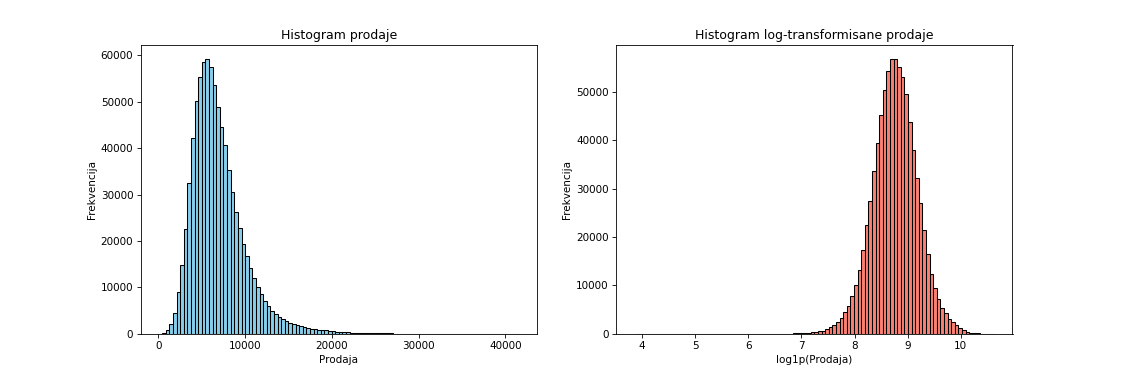
\includegraphics[width=0.85\textwidth]{grafici/sales_histogram.png}
\end{center}

Distribucija prodaje pokazuje izraženu desnu asimetriju, što ukazuje na potrebu za logaritamskom transformacijom ciljne promenljive kako bi se stabilizovala varijansa.

\end{frame}

%---------------------------------
\begin{frame}{Prodaja u zavisnosti od vremena i promocije}
\begin{figure}[H]
    \centering
    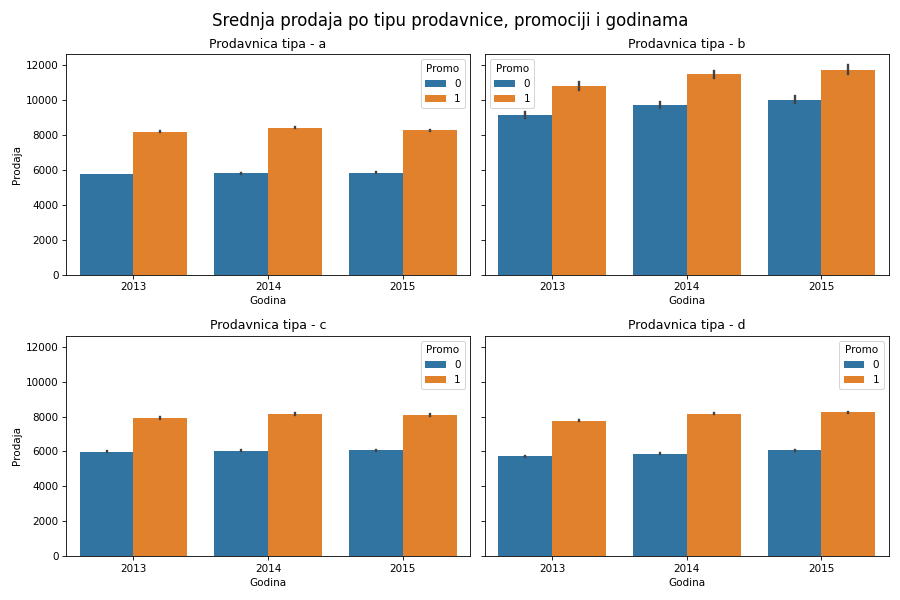
\includegraphics[width=0.32\textwidth]{grafici/promo_by_year.png}
    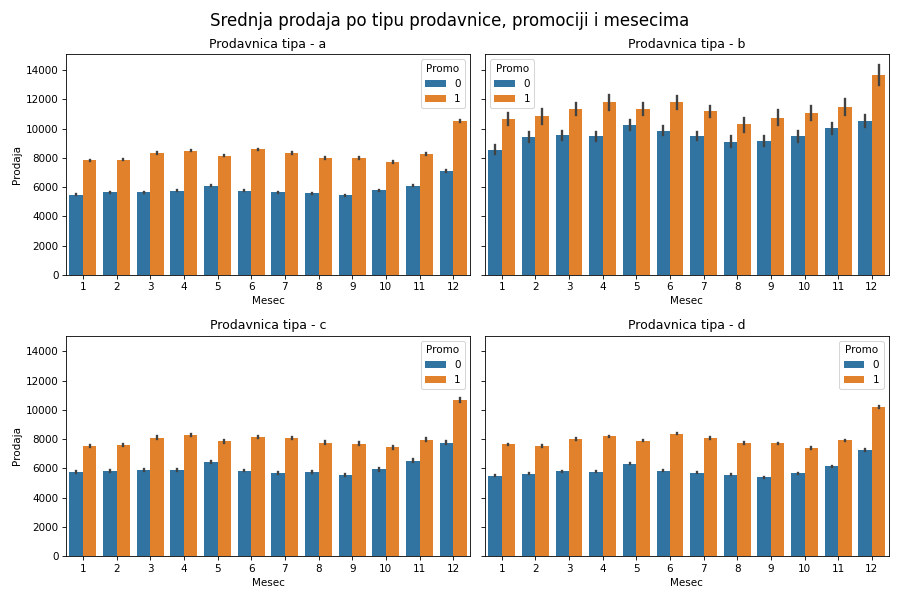
\includegraphics[width=0.32\textwidth]{grafici/promo_by_month.png}
    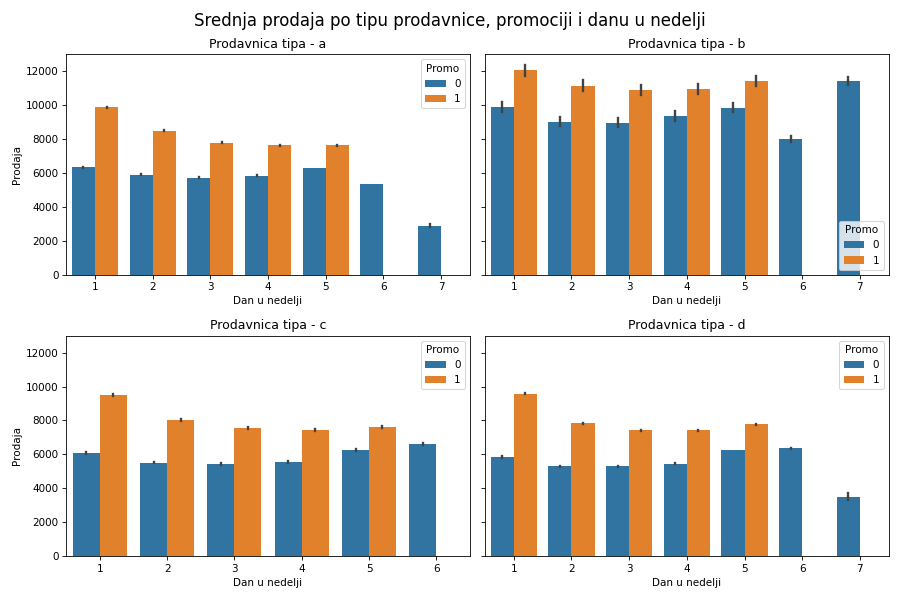
\includegraphics[width=0.32\textwidth]{grafici/promo_by_day.png}
\end{figure}

\begin{itemize}
    \item Vidljiv je sezonski obrazac — porast prodaje u decembru zbog praznika.
    \item Tokom vikenda, većina prodavnica ima smanjenu prodaju.
    \item Promocije značajno povećavaju dnevnu prodaju.
\end{itemize}
\end{frame}

%---------------------------------
\begin{frame}{Uticaj programa Promo2}
\begin{figure}[H]
    \centering
    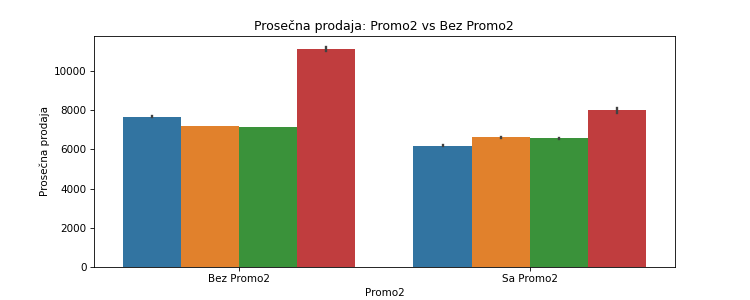
\includegraphics[width=0.48\textwidth]{grafici/promo2_avg_sales.png}
    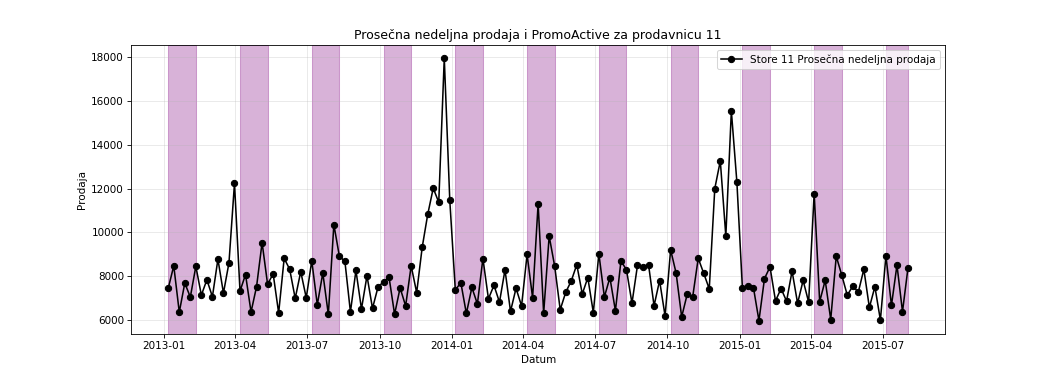
\includegraphics[width=0.48\textwidth]{grafici/promo2_example.png}
\end{figure}

\begin{itemize}
    \item Prodavnice uključene u dugoročne promocije (Promo2) generalno imaju nižu prodaju.
    \item Efekat zavisi od tipa prodavnice – najizraženiji kod tipa „a“ i „d“.
\end{itemize}
\end{frame}

%---------------------------------
\begin{frame}{Uticaj udaljenosti konkurencije}
\begin{figure}[H]
    \centering
    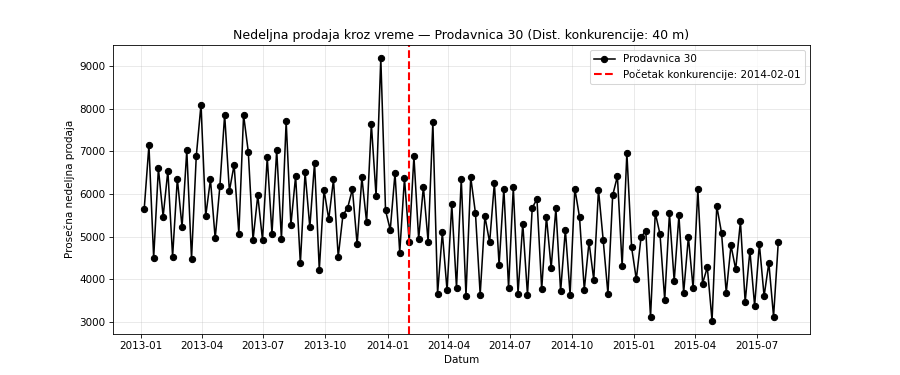
\includegraphics[width=0.48\textwidth]{grafici/competition_near.png}
    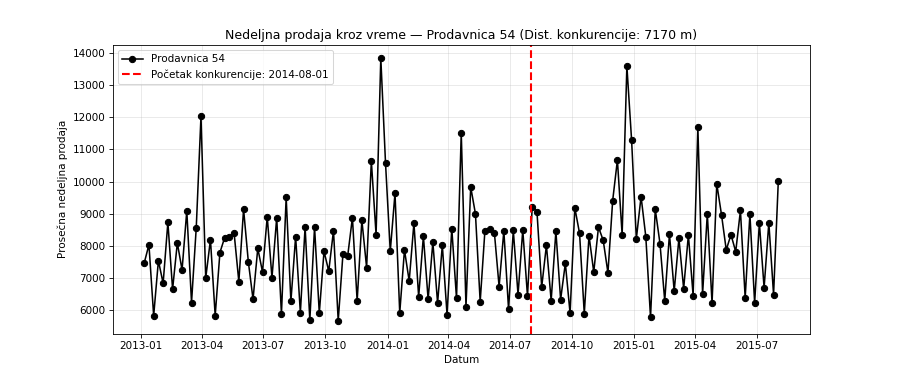
\includegraphics[width=0.48\textwidth]{grafici/competition_far.png}
\end{figure}

\begin{itemize}
    \item Prodavnice sa bližom konkurencijom imaju generalno manju prodaju.
\end{itemize}
\end{frame}

%---------------------------------
\begin{frame}{Uticaj praznika i školskih odmora}
\begin{figure}[H]
    \centering
    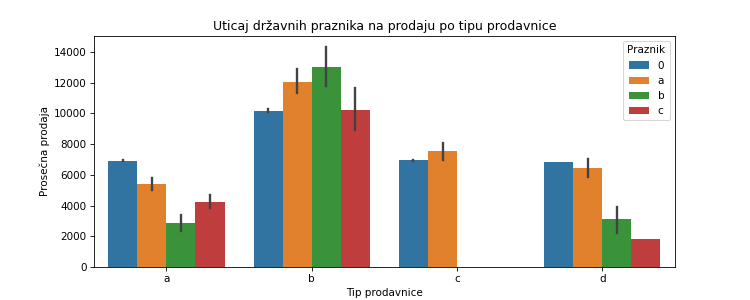
\includegraphics[width=0.48\textwidth]{grafici/holiday_effects.png}
    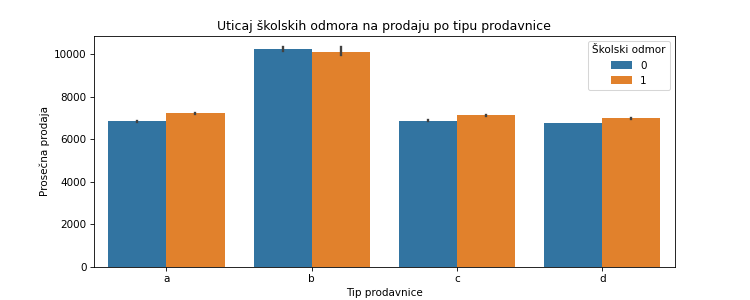
\includegraphics[width=0.48\textwidth]{grafici/school_holidays.png}
\end{figure}

\begin{itemize}
    \item Tokom državnih praznika prodavnice tipa \texttt{b} beleže primetan skok prodaje, dok kod prodavnica tipa \texttt{a} i \texttt{d} dolazi do blagog pada.
    \item Tokom školskih odmora uočava se blag porast prodaje.
\end{itemize}
\end{frame}

%---------------------------------
\begin{frame}{Provera stacionarnosti vremenske serije}
\begin{center}
    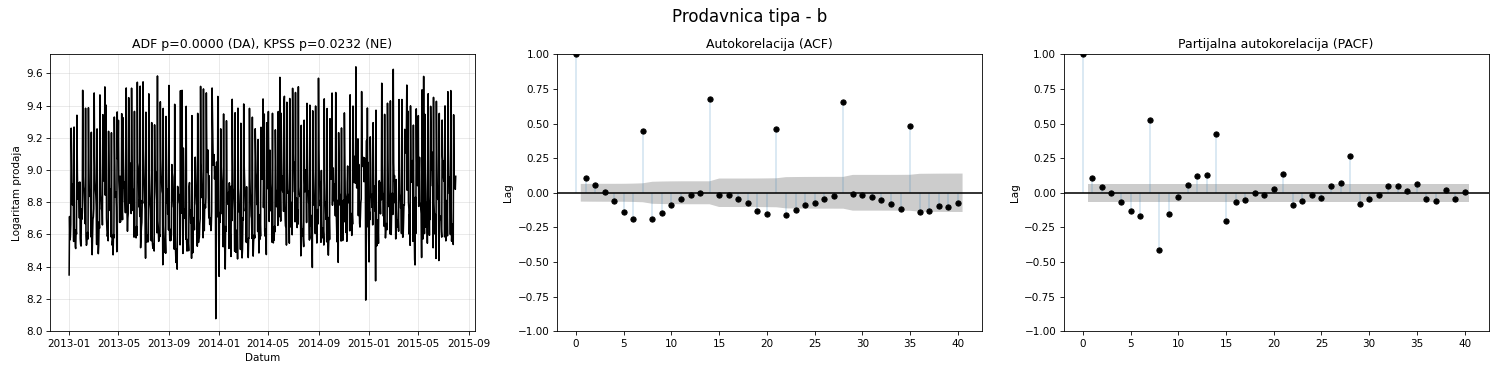
\includegraphics[width=0.85\textwidth]{grafici/store_b.png}
\end{center}

\begin{itemize}
    \item KPSS test ukazuje na prisustvo slučajnog hoda, što znači da se serija ne može smatrati stacionarnom.
    \item Na osnovu ACF i PACF analiza primećeno je da situacija značajno varira u zavisnosti od tipa prodavnice, ali se generalno uočava izražena sezonska komponenta na periodu od 7 do 12 dana.
    \item Kod PACF dijagrama najčešće se ističe autokorelacija sa prethodnim odbirkom ili odbirkom zakašnjenim za 7 dana.
\end{itemize}


\end{frame}

%---------------------------------
\begin{frame}{Detekcija i tretman \textit{outlier}-a}
\begin{figure}[H]
    \centering
    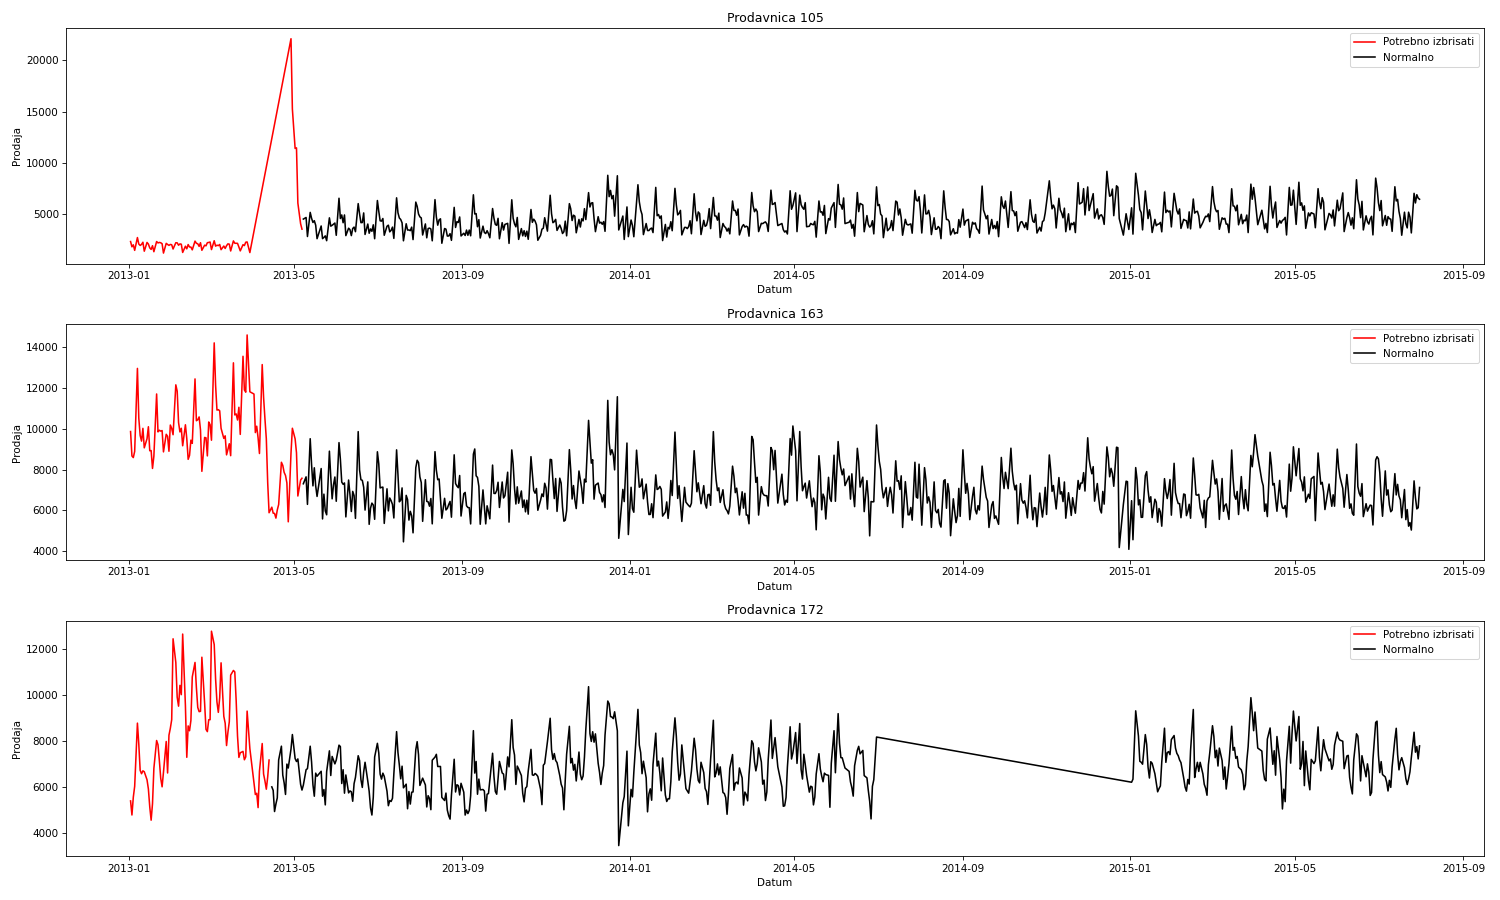
\includegraphics[width=0.42\textwidth]{grafici/outlier_27stores.png}
    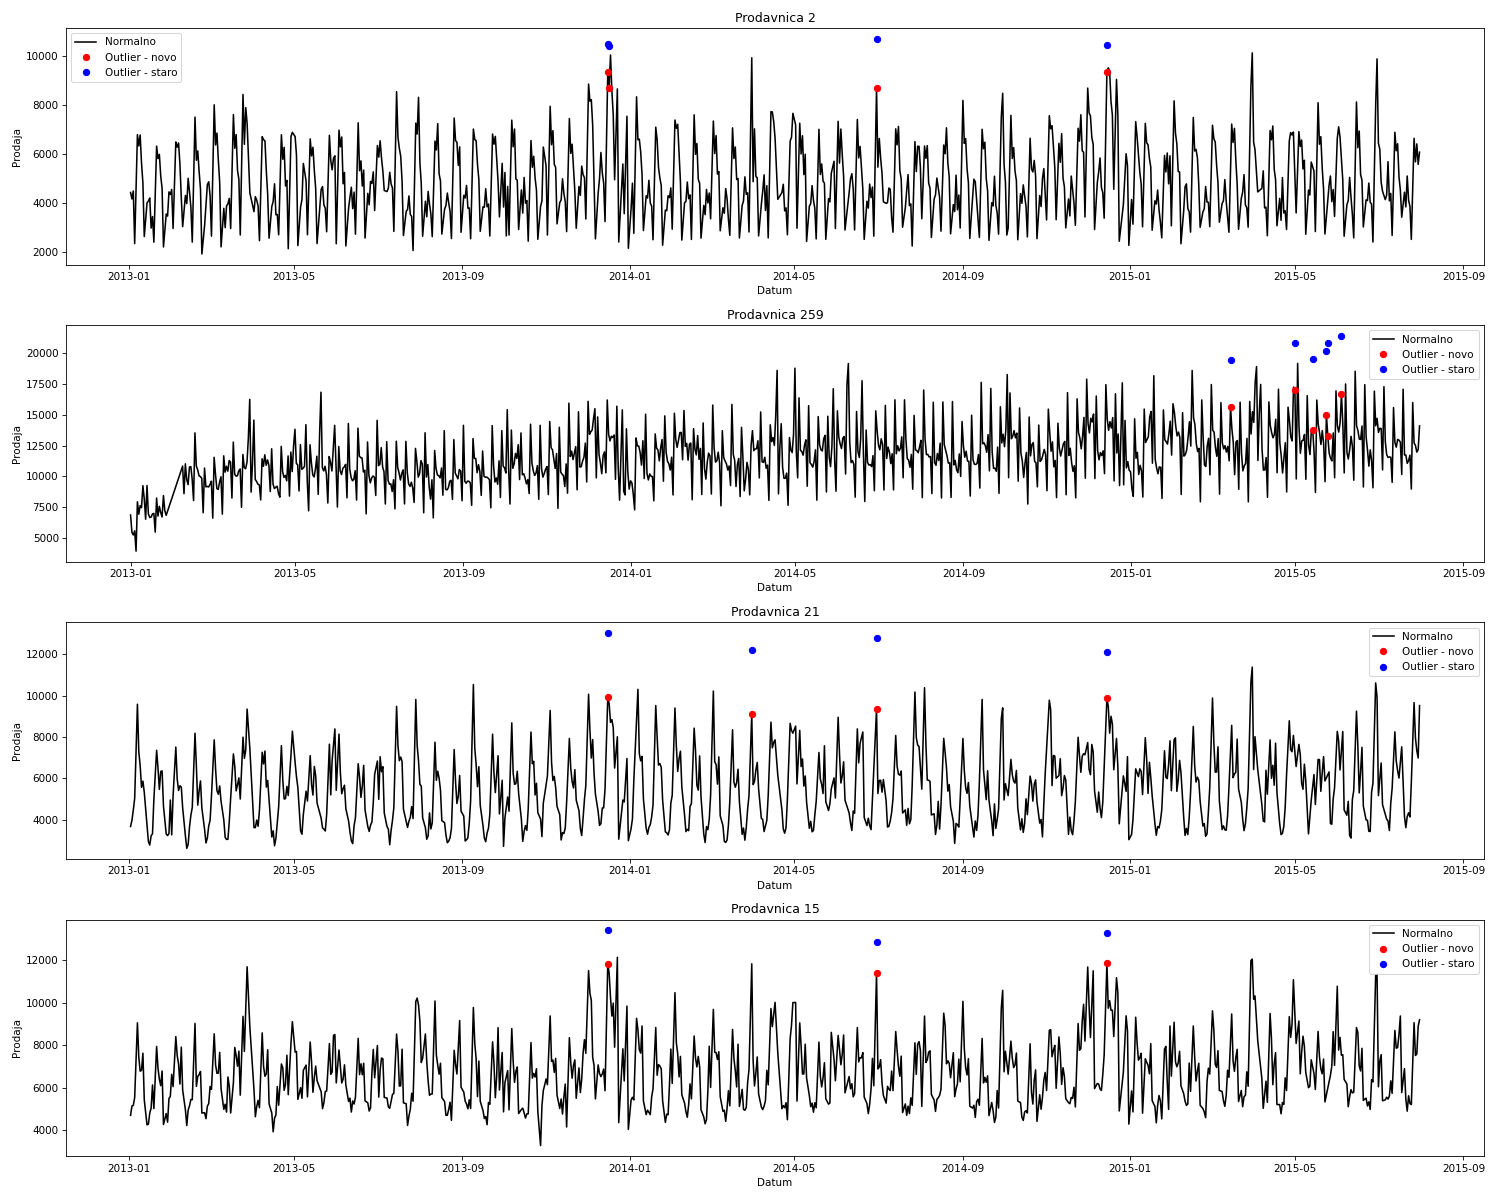
\includegraphics[width=0.42\textwidth]{grafici/outlier_correction.png}
\end{figure}

\begin{itemize}
    \item U početnom periodu primećeno je da pojedine prodavnice pokazuju obrasce prodaje koji se ne mogu objasniti dostupnim obeležjima.
    \item Uočene su ekstremno visoke vrednosti prodaje kod određenih prodavnica, koje mogu negativno uticati na stabilnost i tačnost modela.
\end{itemize}
\end{frame}

\section{Modelovanje}
\begin{frame}{Inženjering karakteristika}
\begin{columns}[T,onlytextwidth]
    % Leva kolona – slika
    \column{0.45\textwidth}
    \begin{figure}[H]
        \centering
        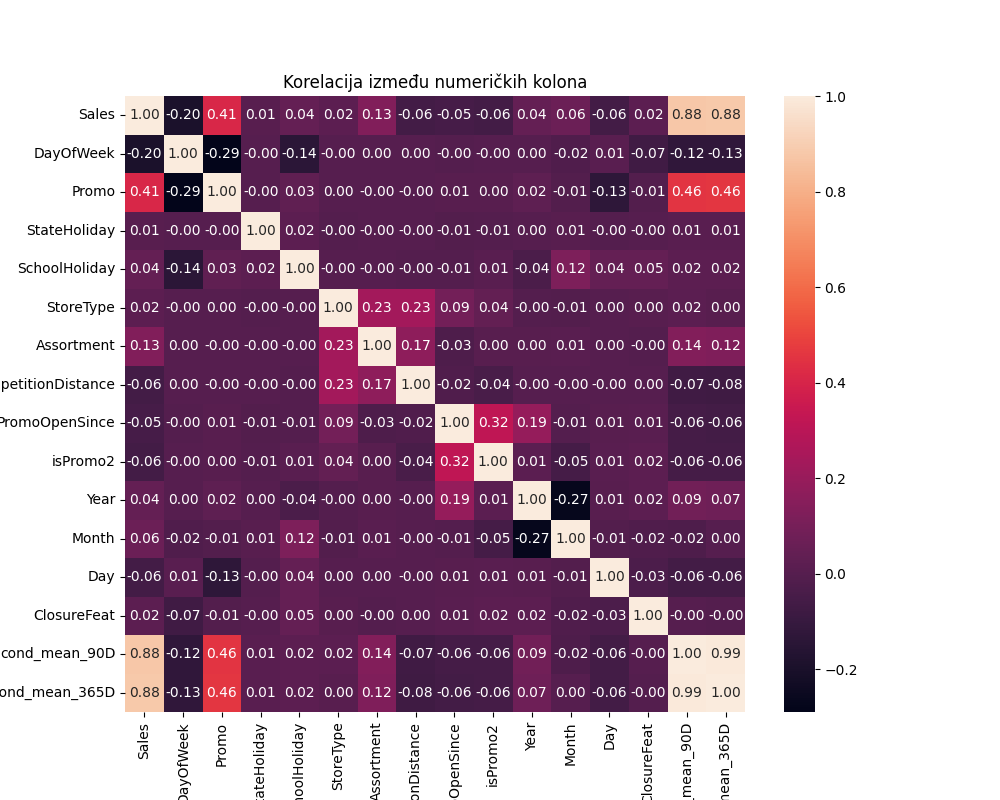
\includegraphics[width=\linewidth]{grafici/correlation_engineered.png}
    \end{figure}

    % Desna kolona – tekst
    \column{0.55\textwidth}
    \begin{itemize}
        \item Dodate su sledeće karakteristike:
        \begin{itemize}
            \item koliko dugo je prisutna konkurencija u okruženju prodavnice,
            \vspace{0.1em}\item trajanje promotivnih perioda,
            \vspace{0.1em}\item informacije o prošlim, sadašnjim i budućim praznicima,
            \vspace{0.1em}\item statističke pokazatelje prodavnice (npr. prosečna prodaja, broj kupaca),
            \vspace{0.1em}\item \textbf{Furijeove komponente} radi hvatanja sezonalnosti.
        \end{itemize}
        
    \end{itemize}
\end{columns}
\end{frame}

\begin{frame}{Modeli}
\begin{itemize}
    \item U radu su korišćena tri pristupa modelovanja:
    \begin{itemize}
        \item \textbf{Konstantan model} – jednostavan bazni koji predviđa prosečnu vrednost prodaje.
        \vspace{0.3em}
        \item \textbf{Ridge regresija} – linearni model sa regularizacijom, primenjen u tri varijante:
        \begin{itemize}
            \item \textit{Globalni model} – jedan model za sve prodavnice.
            \item \textit{Lokalni model} – poseban model za svaku prodavnicu.
            \item \textit{Hibridni model} – kombinacija lokalnog i globalnog pristupa, gde se individualni model svake prodavnice koriguje zajedničkim modelom.
        \end{itemize}

        \item \textbf{XGBoost} – nelinearni ansambl algoritam zasnovan na gradijentnom \textit{boosting}-u stabala odlučivanja.
        \begin{itemize}
            \item Model treniran u \textit{globalnom} i \textit{hibridnom} režimu.
            \item Omogućava modelovanje nelinearnih odnosa i interakcija između obeležja.
        \end{itemize}
    \end{itemize}
\end{itemize}
\end{frame}

\begin{frame}{Evaluacija}
\begin{itemize}

    \vspace{1em}

    \item Za evaluaciju modela korišćena je metrika \textbf{RMSPE} (\textit{Root Mean Square Percentage Error}):
    \[
    RMSPE = \sqrt{\frac{1}{n} \sum_{i=1}^{n} 
    \left( \frac{y_i - \hat{y}_i}{y_i} \right)^2}
    \]

    \item RMSPE bolje odražava relativne greške, posebno kod prodavnica sa različitim nivoima prodaje.
\end{itemize}
\end{frame}

\section{Rezultati}

\begin{frame}{Rezultati modela}
\begin{columns}[T,onlytextwidth]
    % Leva kolona — tabela
    \column{0.55\textwidth}
    \begin{table}[H]
    \centering
    \scriptsize
    \setbeamertemplate{caption}{}
    \caption*{\textbf{Poređenje modela po RMSPE}}
    \begin{tabular}{|l|c|c|c|}
    \hline
    Model & Tip & Public & Test \\ 
    \hline
    Konstantan izlaz & - & 0.27098 & 0.24148 \\ 
    \hline
    \multirow{3}{*}{Ridge} 
        & Globalno & 0.19453 & 0.19839 \\ \cline{2-4}
        & Lokalno & 0.11821 & 0.12940 \\ \cline{2-4}
        & Hibridno & 0.11765 & 0.12807 \\ 
    \hline
    \multirow{2}{*}{XGBoost} 
        & Globalno & 0.10385 & 0.11321 \\ \cline{2-4}
        & Hibridno & 0.10538 & 0.11440 \\ 
    \hline
    \end{tabular}
    \end{table}


    % Desna kolona — komentar rezultata
    \column{0.45\textwidth}
    \begin{itemize}
        \item \textbf{Bazni model} daje očekivano loše rezultate i služi kao referenca.
        \vspace{0.3em}
        \item \textbf{Ridge regresija} značajno poboljšava performanse, posebno u \textit{lokalnom} i \textit{hibridnom} režimu.
        \vspace{0.3em}
        \item \textbf{XGBoost} ostvaruje najbolje rezultate zahvaljujući mogućnosti modelovanja nelinearnih odnosa i interakcija.
    \end{itemize}
\end{columns}
\end{frame}

\begin{frame}{Primer predikcija prodaje po modelima}
    \begin{figure}[H]
        \centering
        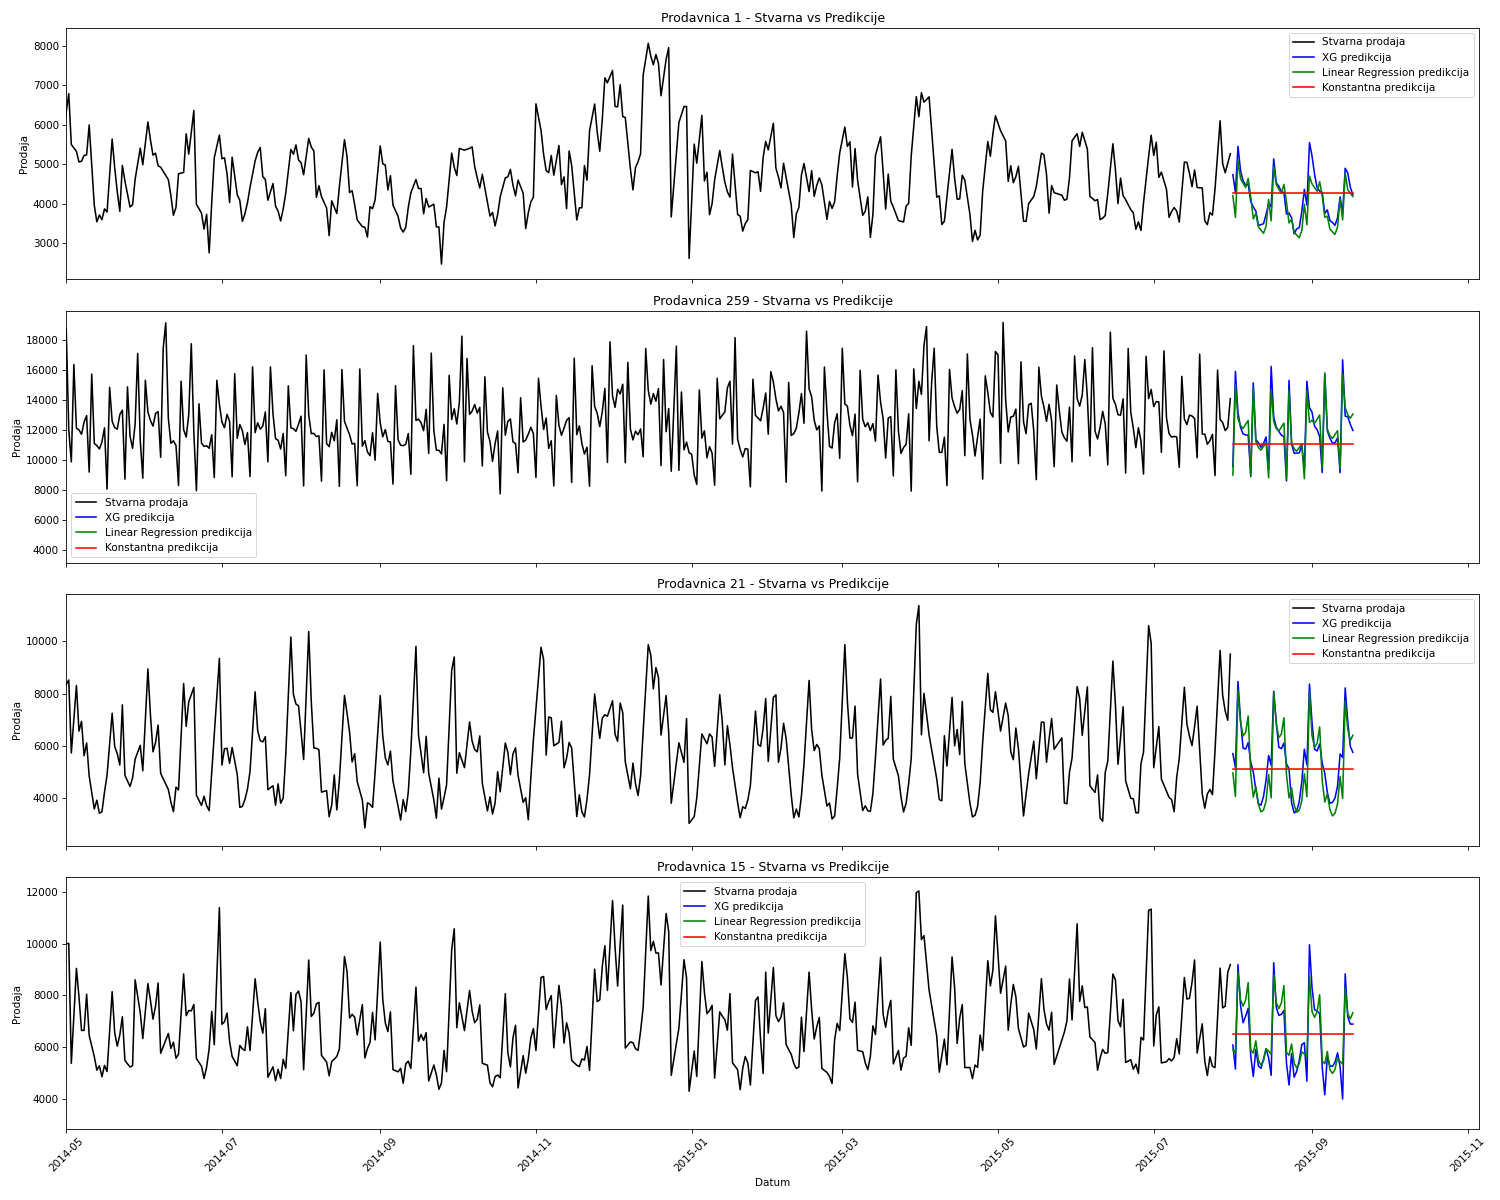
\includegraphics[width=0.6\linewidth]{grafici/prediction_final.png}
    \end{figure}
\end{frame}

\section{Zaključak i dalji pravci}
\begin{frame}{Zaključak i dalji pravci}
\begin{itemize}
    \item Prikazana su tri različita pristupa predikcije prodaje Rossmann prodavnica: konstantan izlaz, Ridge regresija i XGBoost.
    \item Najbolje performanse ostvario je XGBoost zbog sposobnosti modelovanja nelinearnih odnosa i interakcija između promenljivih.
    \item Poređenje sa Kaggle leaderboard-om: pobednički model na privatnom setu ostvario je RMSPE $\approx$ 0.10021. Taj model je koristio i meteorološke podatke, što je tehnički bilo dozvoljeno, ali u realnoj primeni nije uvek praktično, jer je teško precizno predvideti vremenske uslove 6 nedelja unapred.
    \item Preporuke za dalji rad:
    \begin{itemize}
        \item Primena neuralnih  mreža (LSTM, TFT) za vremenske serije.
        \item Uvođenje dodatnih spoljnih faktora: vremenska prognoza, Google Trends.
    \end{itemize}
\end{itemize}
\end{frame}


\end{document}